% !TEX program = xelatex
\documentclass[]{article}
\usepackage{commons/course}

\begin{document}
\printheader

\section*{سوال اول}
\subsection*{قسمت اول}
\begin{gather*}
    S \rightarrow 0S0 | 0S1 | 1S0 | 1S1 | 0
\end{gather*}
\subsection*{قسمت دوم}
\begin{gather*}
    S \rightarrow 0S0 | 1S1 | \epsilon
\end{gather*}
\subsection*{قسمت سوم}
عبارت
$R_i$
یعنی اینکه به
$i$
0 دیگر نیاز داریم
که شرط مسئله ارضا شود.
\begin{align*}
    S &\rightarrow R_3\\
    R_3 &\rightarrow 1R_3 | 0R_2\\
    R_2 &\rightarrow 1R_2 | 0R_1\\
    R_1 &\rightarrow 1R_1 | 0R_0\\
    R_0 &\rightarrow 1R_0 | 0R_0 | \epsilon\\
\end{align*}
\section*{سوال دوم}
\begin{enumerate}
    \item رشته‌هایی که طول آن‌ها فرد است.
    \item $1^a 0^b, \quad a, b \ge 0$
\end{enumerate}
\section*{سوال سوم}
\subsection*{قسمت اول}
برای اینکه مورد خواسته شده در سوال را چک کنیم کافی است برای هر قانون در گرامر شرط‌های زیر را چک
بکنیم: به ازای هر قانون
$A \rightarrow \alpha | \beta$
باید:
\begin{enumerate}
    \item $\operatorname{First}(\alpha) \cap \operatorname{First}(\beta) = \emptyset$
    \item در صورتی که $\alpha \implies^* \epsilon$ آنگاه  $\operatorname{Follow}(\alpha) \cap \operatorname{First}(\beta) = \emptyset$
    \item فقط یکی از عبارت $\alpha \implies^* \epsilon$ و $\beta \implies^* \epsilon$ درست است.
\end{enumerate}
پس در ابتدا
\lr{First}
تمامی
\lr{non terminal}ها
را پیدا می‌کنیم. (مشخص است که \lr{First} همه‌ی \lr{terminal}ها خودشان هستند.)
\begin{align*}
    \operatorname{First}(S) &= \{a\}\\
    \operatorname{First}(A) &= \{a, b\}\\
    \operatorname{First}(B) &= \{\epsilon, a, b\}\\
    \operatorname{First}(C) &= \{b, a\}\\
    \operatorname{First}(D) &= \{d\}
\end{align*}
اما در همان قاعده‌ی اول به مشکل می‌خوریم. چرا که
$\operatorname{First}(aaB)$ و $\operatorname{First}(aAC)$
هر جفتشان
$a$
هستند و در نتیجه نمی‌توان که پیش بینی کرد که باید کدام قاعده را باز کرد.
\subsection*{قسمت دوم}
در ابتدا از قاعده‌ی آخر شروع می‌کنیم که کلا قاعده‌ی اضافی است و هیچ‌جایی استفاده نمی‌شود.
این قاعده عملا زبان
$d^n$
است که پس می‌توان صرفا آن را به صورت
$D \rightarrow dD', D' \rightarrow dD' | \epsilon$
نوشت. حال نکته‌ای که باید به آن توجه بکنید این است که بقیه‌ی قاعده‌ها
\lr{left recursion}
ندارند. حتی اگر قاعده‌ها را دنبال نیز بکنیم باز هم به هیچ
\lr{let recursion}ای
نمی‌رسیم چرا که از سمت چپ نمی‌توان یک
\lr{loop}
زد در
\lr{non terminal}ها.
حال با این موضوع سعی می‌کنیم که با فاکتورگیری از گرامر آن را
predictive
کنیم. در ابتدا دقت کنید که در قانون دوم هر دو طرف می‌توانند که با
$a$
شروع شوند. چرا که می‌توان
$B$ را به $C$ برد و $C$ را به $abc$.
پس عملا با بازنوسی داریم:
\begin{gather*}
    A \rightarrow abcCbCbC | bCbCbC | bC | a
\end{gather*}
پس در اینجا
$a$ و $b$
را فاکتور می‌گیریم.
\begin{align*}
    A  &\rightarrow aA' | bCA''\\
    A' &\rightarrow bcCbCbC | \epsilon\\
    A'' &\rightarrow bCbC | \epsilon
\end{align*}
همان طور که مشاهده می‌شود حال سمت راست قواعد درست شده قابل
\lr{prediction}
هستند. حال سراغ قاعده‌ی
$S$
می‌رویم و
$a$
را فاکتور می‌گیریم.
\begin{align*}
    S &\rightarrow aS'\\
    S' &\rightarrow aB | AC
\end{align*}
اما هنوز کار ما تمام نشده است چرا که
$\operatorname{First}(aB)$ و $\operatorname{First}(AC)$
هر دو
$a$
دارند. در ابتدا دقت کنید که
$S' \rightarrow aB | aA'C | bCA''C$
پس کافی است که یک فاکتور گیری دیگر از
$a$
داشته باشیم:
\begin{align*}
    S &\rightarrow aS'\\
    S' &\rightarrow aS'' | bCA''C\\
    S'' &\rightarrow B | A'C
\end{align*}
حال
$B$ و $A'$
را باز می‌کنیم:
\begin{gather*}
    S'' \rightarrow CCbC | bcCbCbCC | C | \epsilon
\end{gather*}
در نهایت می‌توان
$S''$
را به صورت زیر نوشت:
\begin{align*}
    S'' &\rightarrow abcCbC | bCbC | bcCbCbCC | abc | b | \epsilon\\
    &\implies\\
    S'' &\rightarrow abcS''' | bS'''' | \epsilon\\
    S''' &\rightarrow CbC | \epsilon\\
    S'''' &\rightarrow CbC | cCbCbCC | \epsilon
\end{align*}
پس در نهایت قوانین ما برابر هستند با:
\begin{align*}
    S &\rightarrow aS'\\
    S' &\rightarrow aS'' | bCA''C\\
    S'' &\rightarrow abcS''' | bS'''' | \epsilon\\
    S''' &\rightarrow CbC | \epsilon\\
    S'''' &\rightarrow CbC | cCbCbCC | \epsilon\\
    A  &\rightarrow aA' | bCA''\\
    A' &\rightarrow bcCbCbC | \epsilon\\
    A'' &\rightarrow bCbC | \epsilon\\
    B &\rightarrow CCbC | \epsilon\\
    C &\rightarrow abc | b\\
    D &\rightarrow dD'\\
    D' &\rightarrow dD' | \epsilon
\end{align*}
\section*{سوال چهارم}
\section*{سوال پنجم}
\subsection*{قسمت اول}
در ابتدا بدون ساده سازی تمامی قوانین را می‌نویسیم:
\begin{figure}[H]
    \centering
    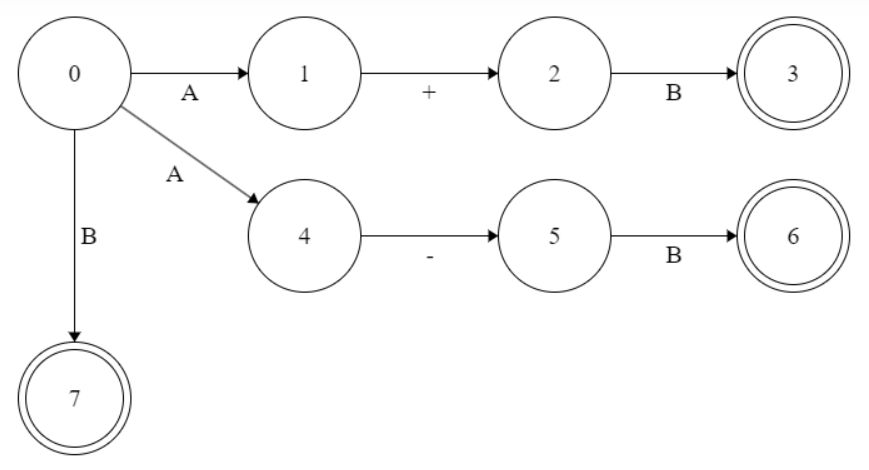
\includegraphics[scale=0.5]{figure/5-1-A.png}
    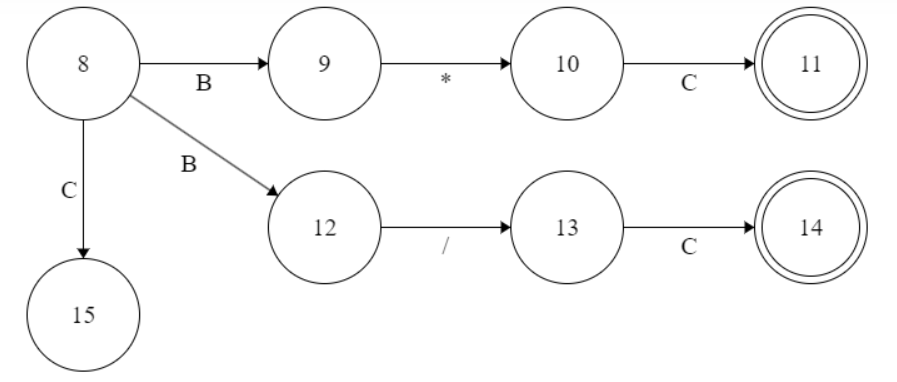
\includegraphics[scale=0.5]{figure/5-1-B.png}
    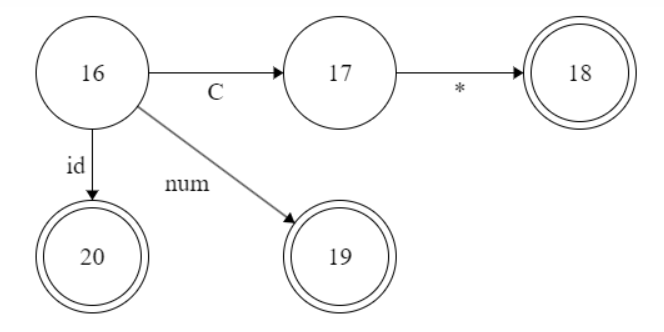
\includegraphics[scale=0.5]{figure/5-1-C.png}
\end{figure}
حال برای ساده سازی هم در ابتدا سعی می‌کنیم حالات تکراری را حذف کنیم.
\begin{figure}[H]
    \centering
    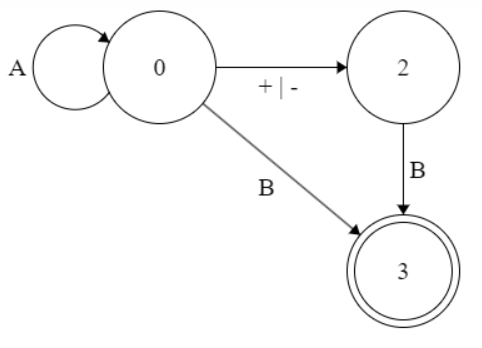
\includegraphics[scale=0.5]{figure/5-1-A-2.png}
    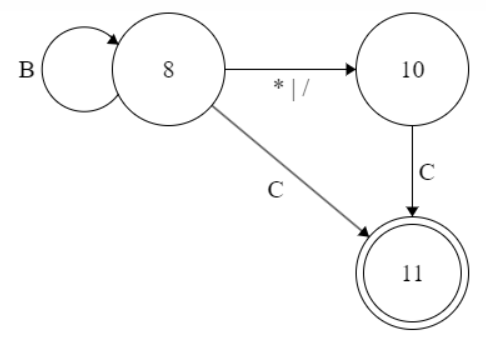
\includegraphics[scale=0.5]{figure/5-1-B-2.png}
    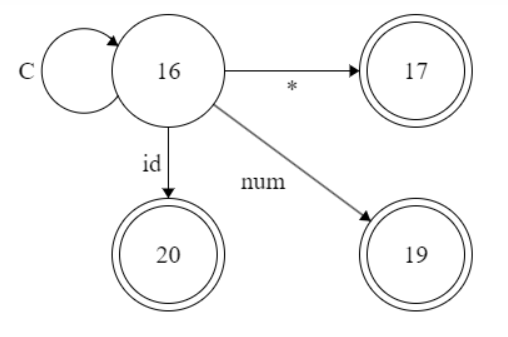
\includegraphics[scale=0.5]{figure/5-1-C-2.png}
\end{figure}
حال از پایین به بالا جایگزاری می‌کنیم. یعنی هر جا در نمودار دوم
$C$
دیدیم
\lr{transition diagram}
آن را قرار می‌دهیم.
\section*{سوال ششم}
\end{document}
